\documentclass[12pt]{article}
\usepackage[utf8]{inputenc}
\usepackage[utf8]{inputenc}
\usepackage{amsmath}
\usepackage{amsthm}
\usepackage{geometry}
\usepackage{amsfonts}
\usepackage{mathrsfs}
\usepackage{bm}
\usepackage{hyperref}
\usepackage[dvipsnames]{xcolor}
\usepackage[inline]{enumitem}
\usepackage{mathtools}
\usepackage{changepage}
\usepackage{lipsum}
\usepackage{tikz}
\usetikzlibrary{matrix, patterns, decorations.pathreplacing, calligraphy}
\usepackage{tikz-cd}
\usepackage[nameinlink]{cleveref}
\geometry{
headheight=15pt,
left=60pt,
right=60pt
}
\setlength{\emergencystretch}{20pt}
\usepackage{fancyhdr}
\pagestyle{fancy}
\fancyhf{}
\lhead{}
\chead{Section 3.2 Exercises}
\rhead{\thepage}
\hypersetup{
    colorlinks=true,
    linkcolor=blue,
    urlcolor=blue
}

\theoremstyle{definition}
\newtheorem*{remark}{Remark}

\newtheoremstyle{exercise}
    {}
    {}
    {}
    {}
    {\bfseries}
    {.}
    { }
    {\thmname{#1}\thmnumber{#2}\thmnote{ (#3)}}
\theoremstyle{exercise}
\newtheorem{exercise}{Exercise 3.2.}

\newtheoremstyle{solution}
    {}
    {}
    {}
    {}
    {\itshape\color{magenta}}
    {.}
    { }
    {\thmname{#1}\thmnote{ #3}}
\theoremstyle{solution}
\newtheorem*{solution}{Solution}

\Crefformat{exercise}{#2Exercise 3.2.#1#3}

\newcommand{\interior}[1]{%
  {\kern0pt#1}^{\mathrm{o}}%
}
\newcommand{\ts}{\textsuperscript}
\newcommand{\setcomp}[1]{#1^{\mathsf{c}}}
\newcommand{\quand}{\quad \text{and} \quad}
\newcommand{\N}{\mathbf{N}}
\newcommand{\Z}{\mathbf{Z}}
\newcommand{\Q}{\mathbf{Q}}
\newcommand{\I}{\mathbf{I}}
\newcommand{\R}{\mathbf{R}}
\newcommand{\C}{\mathbf{C}}

\DeclarePairedDelimiter\abs{\lvert}{\rvert}
% Swap the definition of \abs* and \norm*, so that \abs
% and \norm resizes the size of the brackets, and the 
% starred version does not.
\makeatletter
\let\oldabs\abs
\def\abs{\@ifstar{\oldabs}{\oldabs*}}
%
\let\oldnorm\norm
\def\norm{\@ifstar{\oldnorm}{\oldnorm*}}
\makeatother

\setlist[enumerate,1]{label={(\alph*)}}

\begin{document}

\section{Section 3.2 Exercises}

Exercises with solutions from Section 3.2 of \hyperlink{ua}{[UA]}.

\begin{exercise}
\label{ex:1}
    \begin{enumerate}
        \item Where in the proof of Theorem 3.2.3 part (ii) does the assumption that the collection of open sets be \textit{finite} get used?

        \item Give an example of a countable collection of open sets \( \{ O_1, O_2, O_3, \ldots \} \) whose intersection \( \bigcap_{n=1}^{\infty} O_n \) is closed, not empty and not all of \( \R \).
    \end{enumerate}
\end{exercise}

\begin{solution}
    \begin{enumerate}
        \item This assumption is used when we let \( \epsilon = \min \{ \epsilon_1, \epsilon_2, \ldots, \epsilon_N \} \); this minimum is guaranteed to exist because the set \( \{ \epsilon_1, \epsilon_2, \ldots, \epsilon_N \} \) is finite. An infinite subset of \( \R \) does not necessarily have a minimum. For example, \( \{ n^{-1} : n \in \N \} \) has no minimum.

        \item For each \( n \in \N \), let \( O_n = (-n^{-1}, n^{-1}) \). Then each \( O_n \) is open by Example 3.2.2 (ii), the collection \( \{ O_1, O_2, O_3, \ldots \} \) is countable, and \( \bigcap_{n=1}^{\infty} O_n = \{ 0 \} = [0, 0] \), which is non-empty, not equal to \( \R \), and closed by Example 3.2.9 (ii).
    \end{enumerate}
\end{solution}

\begin{exercise}
\label{ex:2}
    Let
    \[
        A = \left\{ (-1)^n + \frac{2}{n} : n = 1, 2, 3, \ldots \right\} \quand B = \{ x \in \Q : 0 < x < 1 \}.
    \]
    Answer the following questions for each set:
    \begin{enumerate}
        \item What are the limit points?

        \item Is the set open? Closed?

        \item Does the set contain any isolated points?

        \item Find the closure of the set.
    \end{enumerate}
\end{exercise}

\begin{solution}
    Let us consider the set \( A \) first.
    \begin{enumerate}
        \item Let \( L_A \) be the set of limit points of \( A \). We claim that \( L_A = \{ -1, 1 \} \). To see this, let \( (x_n) \) be the sequence given by \( x_n = (-1)^n + 2 n^{-1} \) and consider the subsequences \( (x_{2n+1}) \) and \( (x_{2n}) \). Then:
        \begin{itemize}
            \item each element of \( (x_n) \) belongs to \( A \);

            \item \( \lim_n x_{2n+1} = -1 \);

            \item \( x_{2n+1} \neq -1 \) for each \( n \);

            \item \( \lim_n x_{2n} = 1 \);

            \item \( x_{2n} \neq 1 \) for each \( n \).
        \end{itemize}
        Hence by Theorem 3.2.5, \( -1 \) and \( 1 \) are limit points of \( A \). Now suppose that \( x \in \R \) is such that \( x \neq -1 \) and \( x \neq 1 \), so that \( \epsilon := \min \{ \abs{x + 1}, \abs{x - 1} \} \) is positive. Let \( N \in \N \) be such that \( 2 / N < \epsilon / 2 \). Then for \( n \geq N \) we have
        \[
            (-1)^n + \frac{2}{n} \in \left( -1 - \tfrac{\epsilon}{2}, -1 + \tfrac{\epsilon}{2} \right) \cup \left( 1 - \tfrac{\epsilon}{2}, 1 + \tfrac{\epsilon}{2} \right).
        \]
        It follows that
        \[
            (-1)^n + \frac{2}{n} \not\in \left( x - \tfrac{\epsilon}{2}, x + \tfrac{\epsilon}{2} \right).
        \]

        \begin{figure}[h]
            \centering
            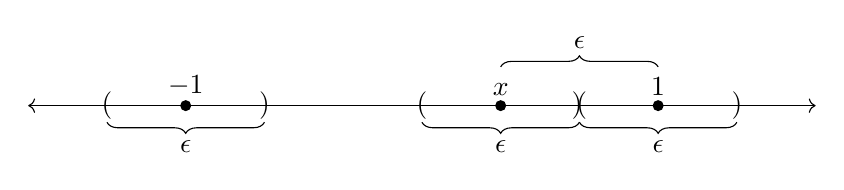
\begin{tikzpicture}
                \draw[<->] (-5,0) -- (5,0);

                \fill (-3,0) circle [radius=0.07] node [anchor=south] {$-1$};
                \fill (3,0) circle [radius=0.07] node [anchor=south] {$1$};
                \fill (1,0) circle [radius=0.07] node [anchor=south] {$x$};

                \node at (-4,0) {(};
                \node at (-2,0) {)};
                \node at (0,0) {(};
                \node at (1.97,0) {)};
                \node at (2.03,0) {(};
                \node at (4,0) {)};

                \draw[decorate, decoration = {brace, raise = 6, amplitude = 4}] (-2,0) -- (-4,0) node [pos = 0.5, below = 9] {\( \epsilon \)};
                \draw[decorate, decoration = {brace, raise = 6, amplitude = 4}] (2,0) -- (0,0) node [pos = 0.5, below = 9] {\( \epsilon \)};
                \draw[decorate, decoration = {brace, raise = 6, amplitude = 4}] (4,0) -- (2,0) node [pos = 0.5, below = 9] {\( \epsilon \)};

                \draw[decorate, decoration = {brace, raise = 14, amplitude = 4}] (1,0) -- (3,0) node [pos = 0.5, above = 17] {\( \epsilon \)};
            \end{tikzpicture}
        \end{figure}

        Thus there can be only finitely many elements of \( A \) in \( V_{\epsilon/2}(x) \); it follows that \( x \) cannot possibly be the limit of any sequence of elements of \( A \) distinct from \( x \), which by Theorem 3.2.5 is to say that \( x \) cannot be a limit point of \( A \). We may conclude that \( L_A = \{ -1, 1 \} \).

        \item \( A \) is not open. To see this, consider the point \( 2 \in A \). We claim that for any \( \epsilon > 0 \), the neighbourhood \( V_{\epsilon}(2) \) contains some \( x \not\in A \), so that \( V_{\epsilon}(2) \not\subseteq A \). It is not hard to see that every element \( a \) of \( A \) other than 2 satisfies \( a \leq 3/2 \). Given this, if we let \( x = 2 + \epsilon / 2 \) then \( x \in V_{\epsilon}(2) \) and \( x \not\in A \).

        \( A \) is not closed either since it does not contain the limit point \( -1 \); for any \( n \in \N \) we have \( (-1)^n + 2 / n > -1 \).

        \item Since \( L_A = \{ -1, 1 \}, 1 \in A \) and \( -1 \not\in A \), every point of \( A \) other than \( 1 \) is an isolated point of \( A \).

        \item The closure is
        \[
            \overline{A} = A \cup L_A = \{ -1 \} \cup \left\{ (-1)^n + \frac{2}{n} : n = 1, 2, 3, \ldots \right\}.
        \]
    \end{enumerate}

    Now let us consider the set \( B \).
    \begin{enumerate}
        \item Let \( L_B \) be the set of limit points of \( B \). We claim that \( L_B = [0, 1] \). To see this, first suppose that \( x \in [0, 1] \) and let \( \epsilon > 0 \) be given. Observe that
        \[
            V_{\epsilon}(x) \cap (0, 1) = (\max \{ x - \epsilon, 0 \}, \min \{ x + \epsilon, 1 \}).
        \]
        This is a proper interval contained in \( (0, 1) \) and hence contains infinitely many elements of \( B \). It follows that \( x \) is a limit point of \( B \) and hence that \( [0, 1] \subseteq L_B \).
        
        If \( x \) is a limit point of \( B \) then by Theorem 3.2.5 it must be the case that \( x \) is the limit of a sequence of elements of \( B \). The Order Limit Theorem then implies that \( 0 \leq x \leq 1 \), so that \( L_B \subseteq [0, 1] \). We may conclude that \( L_B = [0, 1] \).

        \item \( B \) is not open, since for any \( x \in B \) and \( \epsilon > 0 \), the set \( V_{\epsilon}(x) \) will contain irrational numbers and hence cannot be contained in \( B \). \( B \) is also not closed, since it does not contain the limit point \( 0 \).

        \item \( B \) does not contain any isolated points, since \( B \subseteq L_B = [0, 1] \).

        \item We have \( \overline{B} = B \cup L_B = L_B = [0, 1] \).
    \end{enumerate}
\end{solution}

\begin{exercise}
\label{ex:3}
    Decide whether the following sets are open, closed, or neither. If a set is not open, find a point in the set for which there is no \( \epsilon \)-neighborhood contained in the set. If a set is not closed, find a limit point that is not contained in the set.
    \begin{enumerate}
        \item \( \Q \).

        \item \( \N \).

        \item \( \{ x \in \R : x \neq 0 \} \).

        \item \( \{ 1 + 1/4 + 1/9 + \cdots + 1/n^2 : n \in \N \} \).

        \item \( \{ 1 + 1/2 + 1/3 + \cdots + 1/n : n \in \N \} \).
    \end{enumerate}
\end{exercise}

\begin{solution}
    \begin{enumerate}
        \item \( \Q \) is neither open nor closed. To see that \( \Q \) fails to be open, observe that for any \( \epsilon > 0 \) there are infinitely many irrational numbers in \( V_{\epsilon}(0) = (-\epsilon, \epsilon) \). Thus \( V_{\epsilon}(0) \) cannot be contained in \( \Q \). To see that \( \Q \) fails to be closed, observe that \( \sqrt{2} \not\in \Q \) is a limit point of \( \Q \) (Theorem 3.2.10).

        \item \( \N \) is closed but not open. To see that \( \N \) is not open, observe that for any \( \epsilon > 0 \) there are infinitely many non-integers in \( V_{\epsilon}(1) = (1 - \epsilon, 1 + \epsilon) \). It follows that \( V_{\epsilon}(1) \) cannot be contained in \( \N \). To see that \( \N \) is closed, we will show that \( \setcomp{\N} \) is open and appeal to Theorem 3.2.13. Note that
        \[
            \setcomp{\N} = (-\infty, 1) \cup \bigcup_{n=1}^{\infty} (n, n + 1).
        \]
        As shown in Example 3.2.2 (ii), \( (n, n + 1) \) is open for each \( n \in \N \), and it is not hard to see that \( (-\infty, 1) \) is also open. Theorem 3.2.3 (i) then implies that \( \setcomp{\N} \) is open.

        \item Let \( E \) be the set in question. \( E \) is open since it is the union of two open sets, \( E = (-\infty, 0) \cup (0, \infty) \), and \( E \) is not closed since it does not contain the limit point \( 0 \): \( 1/n \to 0 \) and \( 1/n \in E \) for each \( n \in \N \).

        \item Let \( E \) be the set in question. First we claim that \( E \) is not open. To see this, let \( \epsilon > 0 \) be given and note that each element of \( x \in E \) satisfies \( x \geq 1 \). It follows that \( V_{\epsilon}(1) \) cannot be contained in \( E \), since it contains infinitely many real numbers \( x < 1 \). We claim that \( E \) is also not closed. From Chapter 2, we know that \( 1 + 1/4 + 1/9 + \cdots \) converges to some \( L \in \R \). It is then clear that \( L \) is a limit point of \( E \). Observe that for any \( n \in \N \)
        \[
            L - \sum_{j=1}^n \frac{1}{j^2} = \sum_{j=n+1}^{\infty} \frac{1}{j^2} > \frac{1}{(n+1)^2} > 0.
        \]
        It follows that \( L \not\in E \) and hence that \( E \) is not closed.

        \item Let \( E \) be the set in question. The reasoning used in part (d) shows that \( E \) is not open, however we claim that \( E \) is closed. Let \( s_n = \sum_{j=1}^n 1/j \), so that \( E = \{ s_n : n \in \N \} \), and let \( x \in \R \) be given; we will show that \( x \) cannot be a limit point of \( E \). First suppose that \( x \not\in E \). From Chapter 2, we know that \( (s_n) \) is strictly increasing and unbounded. Given this, there exists an \( N \in \N \) such that
        \[
            n \geq N \implies s_n > x + 1.
        \]
        Set \( \epsilon := \min \{ \abs{x - s_1}, \ldots, \abs{x - s_{N-1}}, 1 \} \). Then \( \epsilon \) is positive and
        \[
            n \geq N \implies \abs{x - s_n} > 1 \geq \epsilon \quand n < N \implies \abs{x - s_n} \geq \epsilon.
        \]
        It follows that \( V_{\epsilon}(x) \) does not intersect \( E \) and hence that \( x \) is not a limit point of \( E \). Now suppose that \( x \in E \), so that \( x = s_n \) for some \( n \in \N \). Set
        \[
            \epsilon := s_n - s_{n-1} = \frac{1}{n} > \frac{1}{n+1} = s_{n+1} - s_n > 0.
        \]
        Then since
        \[
            s_1 < \cdots < s_{n-1} < x = s_n < s_{n+1} < \cdots,
        \]
        we have \( V_{\epsilon}(x) \cap E = \{ x \} \). Thus \( x \) is not a limit point of \( E \).

        We have shown that \( E \) has no limit points. It follows that \( E \) vacuously contains all of its limit points and hence is closed.
    \end{enumerate}
\end{solution}

\begin{exercise}
\label{ex:4}
    Let \( A \) be nonempty and bounded above so that \( s = \sup A \) exists.
    \begin{enumerate}
        \item Show that \( s \in \overline{A} \).

        \item Can an open set contain its supremum?
    \end{enumerate}
\end{exercise}

\begin{solution}
    \begin{enumerate}
        \item If \( s \in A \) then certainly \( s \in \overline{A} \), so suppose that \( s \not\in A \). By Lemma 1.3.8, for each \( n \in \N \) we may choose some \( a_n \in A \) satisfying \( s - \tfrac{1}{n} < a_n < s \). The Squeeze Theorem then implies that \( \lim a_n = s \) and so \( s \) is a limit point of \( A \) by Theorem 3.2.5, whence \( s \in \overline{A} \).

        \item An open set cannot contain its supremum. To see this, suppose that \( A \) is open and \( s := \sup A \) belongs to \( A \). There then exists an \( \epsilon > 0 \) such that \( V_{\epsilon}(s) \subseteq A \), which implies that \( s + \epsilon / 2 \in A \), contradicting the fact that \( s \) is the supremum of \( A \).
    \end{enumerate}
\end{solution}

\begin{exercise}
\label{ex:5}
    Prove Theorem 3.2.8.
\end{exercise}

\begin{solution}
    Theorem 3.2.8 states that a set \( F \subseteq \R \) is closed if and only if every Cauchy sequence contained in \( F \) has a limit that is also an element of \( F \). To prove this, first suppose that \( F \subseteq \R \) is closed and let \( (x_n) \) be a Cauchy sequence contained in \( F \). By completeness, we have \( \lim x_n = x \) for some \( x \in \R \). If \( x \in F \) then we are done, otherwise if \( x \not\in F \) then we have \( x_n \neq x \) for all \( n \in \N \), since \( (x_n) \) is contained in \( F \). Theorem 3.2.5 then implies that \( x \) is a limit point of \( F \) and hence belongs to \( F \) since \( F \) is closed.

    Conversely, suppose that every Cauchy sequence contained in \( F \) has a limit that is also an element of \( F \) and let \( x \in \R \) be a limit point of \( F \). By Theorem 3.2.5, there is a sequence \( (x_n) \) contained in \( F \) such that \( \lim x_n = x \) and \( x_n \neq x \) for each \( n \in \N \). Since convergent sequences are also Cauchy sequences, by assumption we then have \( x \in F \). So \( F \) contains all of its limit points and hence is closed.
\end{solution}

\begin{exercise}
\label{ex:6}
    Decide whether the following statements are true or false. Provide counterexamples for those that are false, and supply proofs for those that are true.
    \begin{enumerate}
        \item An open set that contains every rational number must necessarily be all of \( \R \).

        \item The Nested Interval Property remains true if the ``closed interval'' is replaced by ``closed set''.

        \item Every nonempty open set contains a rational number.

        \item Every bounded infinite closed set contains a rational number.

        \item The Cantor set is closed.
    \end{enumerate}
\end{exercise}

\begin{solution}
    \begin{enumerate}
        \item This is false. Consider the set \( \R \setminus \left\{ \sqrt{2} \right\} = \left( -\infty, \sqrt{2} \right) \cup \left( \sqrt{2}, \infty \right) \). This contains every rational number and is an open set since it is the union of two open sets.
        
        \item This is false. For a counterexample, consider the closed sets \( [n, \infty) \) for \( n \in \N \) (it is not hard to see that for any \( a \in \R \), the set \( [a, \infty) \) is closed). These sets are nested, however
        \[
            \bigcap_{n=1}^{\infty} [n, \infty) = \emptyset.
        \]

        \item This is true. Suppose that \( A \) is open and non-empty, so that there exists some \( x \in A \). There is then an \( \epsilon > 0 \) such that \( V_{\epsilon}(x) \subseteq A \). By the density of \( \Q \) in \( \R \), there are infinitely many rational numbers contained in \( V_{\epsilon}(x) \) and hence in \( A \).

        \item This is false. Consider the set
        \[
            E = \left\{ \sqrt{2} \right\} \cup \left\{ \sqrt{2} + \frac{\sqrt{2}}{n} : n \in \N \right\}.
        \]
        This is a bounded infinite set which contains only irrational numbers. Similar reasoning to \Cref{ex:2} (a) shows that \( \sqrt{2} \) is the only limit point of \( E \), which belongs to \( E \). Hence \( E \) is closed.

        \item This is true. Since each \( C_n \) is the union of \( 2^n \) closed intervals, Theorem 3.2.14 (i) shows that each \( C_n \) is closed. Then since \( C = \bigcap_{n=1}^{\infty} C_n \), Theorem 3.2.14 (ii) shows that \( C \) is closed.
    \end{enumerate}
\end{solution}

\begin{exercise}
\label{ex:7}
    Given \( A \subseteq \R \), let \( L \) be the set of all limit points of \( A \).
    \begin{enumerate}
        \item Show that the set \( L \) is closed.

        \item Argue that if \( x \) is a limit point of \( A \cup L \), then \( x \) is a limit point of \( A \). Use this observation to furnish a proof for Theorem 3.2.12.
    \end{enumerate}
\end{exercise}

\begin{solution}
    \begin{enumerate}
        \item Suppose that \( x \in \R \) is a limit point of \( L \); we will show that \( x \) is a limit point of \( A \) also. Let \( \epsilon > 0 \) be given. There exists a \( y \in L, y \neq x \) such that \( \abs{x - y} < \epsilon / 2 \). Since \( y \) is a limit point of \( A \), there also exists an \( a \in A, a \neq y \) such that \( \abs{a - y} < \epsilon / 2 \). It follows that
        \[
            a \in A, a \neq x \quand \abs{a - x} \leq \abs{a - y} + \abs{x - y} < \epsilon / 2 + \epsilon / 2 = \epsilon.
        \]
        Hence \( x \) is a limit point of \( A \), i.e.\ \( x \in L \). So we have shown that \( L \) contains all of its limit points and hence is closed.

        \item Let \( \epsilon > 0 \) be given. Since \( x \) is a limit point of \( A \cup L \), the neighbourhood \( V_{\epsilon/2}(x) \) contains some \( y \in A \cup L \) such that \( y \neq x \). If \( y \in A \), then \( V_{\epsilon}(x) \) contains a point of \( A \) other than \( x \). If \( y \in L \), then the argument given in part (a) shows that \( V_{\epsilon}(x) \) contains a point of \( A \) other than \( x \) in this case also. It follows that \( x \) is a limit point of \( A \).

        This shows that \( \overline{A} = A \cup L \) contains all of its limit points and hence is closed.
    \end{enumerate}
\end{solution}

\begin{exercise}
\label{ex:8}
    Assume \( A \) is an open set and \( B \) is a closed set. Determine if the following sets are definitely open, definitely closed, both, or neither.
    \begin{enumerate}
        \item \( \overline{A \cup B} \)

        \item \( A \setminus B = \{ x \in A : x \not\in B \} \)

        \item \( \setcomp{(\setcomp{A} \cup B)} \)

        \item \( (A \cap B) \cup (\setcomp{A} \cap B) \)

        \item \( \setcomp{\overline{A}} \cap \overline{\setcomp{A}} \)
    \end{enumerate}
\end{exercise}

\begin{solution}
    \begin{enumerate}
        \item \( \overline{A \cup B} \) is definitely closed, by Theorem 3.2.12. It may or may not be open. For example, if \( A = B = \R \), then \( \overline{A \cup B} = \R \) is open. If \( A = (0, 1) \) and \( B = [0, 1] \), then \( \overline{A \cup B} = [0, 1] \) is not open.

        \item Since \( A \setminus B = A \cap \setcomp{B} \) is the intersection of two open sets, \( A \setminus B \) is definitely open. It may or may not be closed. For example, if \( A = (0, 1) \) and \( B = [0, 1] \), then \( A \setminus B = \emptyset \) is closed. If \( A = (0, 1) \) and \( B = [2, 3] \), then \( A \setminus B = (0, 1) \) is not closed.

        \item \( \setcomp{A} \cup B \) is the union of two closed sets and hence is closed. The complement \( \setcomp{(\setcomp{A} \cup B)} \) is then definitely open. It may or may not be closed. For example, if \( A = B = \R \), then \( \setcomp{(\setcomp{A} \cup B)} = \setcomp{(\emptyset \cup \R)} = \setcomp{\R} = \emptyset \) is closed. If \( A = (0, 1) \) and \( B = \setcomp{A} = (-\infty, 0] \cup [1, \infty) \), then
        \[
            \setcomp{(\setcomp{A} \cup B)} = \setcomp{(\setcomp{A} \cup \setcomp{A})} = \setcomp{(\setcomp{A})} = A
        \]
        is not closed.

        \item This is simply the set \( B \), which is given as definitely closed. It may or may not be open; \( B = \R \) is closed and open, whereas \( B = [0, 1] \) is closed but not open.

        \item We claim that \( \setcomp{\overline{A}} \) is a subset of \( \overline{\setcomp{A}} \). To see this, let \( L_A \) be the set of limit points of \( A \) and let \( L_{\setcomp{A}} \) be the set of limit points of \( \setcomp{A} \). Then
        \[
            \setcomp{\overline{A}} = \setcomp{(A \cup L_A)} = \setcomp{A} \cap \setcomp{L_A} \quand \overline{\setcomp{A}} = \setcomp{A} \cup L_{\setcomp{A}}.
        \]
        Our claim now follows since \( \setcomp{\overline{A}} \subseteq \setcomp{A} \subseteq \overline{\setcomp{A}} \). Given this, we have \( \setcomp{\overline{A}} \cap \overline{\setcomp{A}} = \setcomp{\overline{A}} \), which is the complement of a closed set and hence is definitely open. It may or may not be closed. For example, if \( A = \emptyset \), then \( \setcomp{\overline{A}} = \setcomp{\emptyset} = \R \) is closed. If \( A = (-\infty, 0) \), then \( \setcomp{\overline{A}} = \setcomp{(-\infty, 0]} = (0, \infty) \) is not closed.
    \end{enumerate}
\end{solution}

\begin{exercise}[De Morgan's Laws]
\label{ex:9}
    A proof for De Morgan's Laws in the case of two sets is outlined in \href{https://lew98.github.io/Mathematics/UA_Section_1_2_Exercises.pdf}{Exercise 1.2.5}. The general argument is similar.
    \begin{enumerate}
        \item Given a collection of sets \( \{ E_{\lambda} : \lambda \in \Lambda \} \), show that
        \[
            \setcomp{\left( \bigcup_{\lambda \in \Lambda} E_{\lambda} \right)} = \bigcap_{\lambda \in \Lambda} \setcomp{E_{\lambda}} \quand \setcomp{\left( \bigcap_{\lambda \in \Lambda} E_{\lambda} \right)} = \bigcup_{\lambda \in \Lambda} \setcomp{E_{\lambda}}.
        \]

        \item Now, provide the details for the proof of Theorem 3.2.14.
    \end{enumerate}
\end{exercise}

\begin{solution}
    \begin{enumerate}
        \item We have
        \begin{align*}
            x \in \setcomp{\left( \bigcup_{\lambda \in \Lambda} E_{\lambda} \right)} &\iff x \not\in \bigcup_{\lambda \in \Lambda} E_{\lambda} \\[2mm]
            &\iff x \not\in E_{\lambda} \text{ for all } \lambda \in \Lambda \\[2mm]
            &\iff x \in \setcomp{E_{\lambda}} \text{ for all } \lambda \in \Lambda \\[2mm]
            &\iff x \in \bigcap_{\lambda \in \Lambda} \setcomp{E_{\lambda}}.
        \end{align*}
        The equality \( \setcomp{\left( \bigcup_{\lambda \in \Lambda} E_{\lambda} \right)} = \bigcap_{\lambda \in \Lambda} \setcomp{E_{\lambda}} \) follows. Similarly,
        \begin{align*}
            x \in \setcomp{\left( \bigcap_{\lambda \in \Lambda} E_{\lambda} \right)} &\iff x \not\in \bigcap_{\lambda \in \Lambda} E_{\lambda} \\[2mm]
            &\iff x \not\in E_{\lambda'} \text{ for some } \lambda' \in \Lambda \\[2mm]
            &\iff x \in \setcomp{E_{\lambda'}} \text{ for some } \lambda' \in \Lambda \\[2mm]
            &\iff x \in \bigcup_{\lambda \in \Lambda} \setcomp{E_{\lambda}}.
        \end{align*}
        Thus \( \setcomp{\left( \bigcap_{\lambda \in \Lambda} E_{\lambda} \right)} = \bigcup_{\lambda \in \Lambda} \setcomp{E_{\lambda}} \).

        \item Suppose we have finitely many closed sets \( E_1, \ldots, E_n \) and let \( E = E_1 \cup \cdots \cup E_n \). Then by part (a), we have
        \[
            \setcomp{E} = \setcomp{(E_1 \cup \cdots \cup E_n)} = \setcomp{E_1} \cap \cdots \cap \setcomp{E_n}.
        \]
        Each \( \setcomp{E_i} \) is open, so Theorem 3.2.3 (ii) implies that \( \setcomp{E} \), which is a finite intersection of open sets, is also open. It follows that \( E \) is closed. Now suppose that we have an arbitrary collection \( \{ E_{\lambda} : \lambda \in \Lambda \} \) of closed sets and let \( E = \bigcap_{\lambda \in \Lambda} E_{\lambda} \). By part (a), we have
        \[
            \setcomp{E} = \setcomp{\left( \bigcap_{\lambda \in \Lambda} E_{\lambda} \right)} = \bigcup_{\lambda \in \Lambda} \setcomp{E_{\lambda}}.
        \]
        Each \( \setcomp{E_{\lambda}} \) is open, so Theorem 3.2.3 (i) implies that \( \setcomp{E} \), which is an arbitrary union of open sets, is also open. It follows that \( E \) is closed.
    \end{enumerate}
\end{solution}

\begin{exercise}
\label{ex:10}
    Only one of the following three descriptions can be realized. Provide an example that illustrates the viable description, and explain why the other two cannot exist.
    \begin{enumerate}
        \item A countable set contained in \( [0, 1] \) with no limit points.

        \item A countable set contained in \( [0, 1] \) with no isolated points.

        \item A set with an uncountable number of isolated points.
    \end{enumerate}
\end{exercise}

\begin{solution}
    \begin{enumerate}
        \item This is impossible. Suppose that \( E \subseteq [0, 1] \) is countable. Then we may choose a sequence \( (x_n) \) with distinct elements (i.e.\ \( x_n \neq x_m \) for \( n \neq m \)) entirely contained in \( E \). This sequence is certainly bounded, so the Bolzano-Weierstrass Theorem implies that there is a convergent subsequence \( (x_{n_k}) \to x \) for some \( x \in [0, 1] \). Theorem 3.2.5 then implies that \( x \) is a limit point of \( E \). (If \( x_{n_k} = x \) for some \( k \in \N \), simply remove this term from the sequence; there can be at most one such \( k \) since the elements of \( (x_n) \) are distinct, so this will not affect the convergence of the subsequence.)

        \item This is possible. Consider the countable set \( B = (0, 1) \cap \Q \) from \Cref{ex:2}. We showed there that \( B \) has no isolated points.

        \item This is impossible. Suppose that \( E \) is a subset of \( \R \) and let \( A \) be the set of isolated points of \( E \). If \( x \in A \), then there is an \( \epsilon > 0 \) such that \( V_{\epsilon}(x) \cap E = \{ x \} \). By the density of \( \Q \) in \( \R \), there exist rational numbers \( p, q \) such that \( x - \epsilon < p < x < q < x + \epsilon \). Then if we let \( U_x = (p, q) \), it follows that \( U_x \cap E = \{ x \} \). Define \( f : A \to B \) by \( f(x) = U_x \), where
        \[
            B = \bigcup_{p, q \in \Q \text{ with } p < q} \{ (p, q) \}.
        \]
        Theorem 1.5.8 (ii) shows that \( B \) is a countable set. If we assume that \( A \) is uncountable, then the function \( f \) cannot possibly be injective. Therefore there must exist \( x \neq y \) in \( A \) such that \( f(x) = f(y) \), i.e.\ \( U_x = U_y \). This implies that
        \[
            \{ x \} = U_x \cap E = U_y \cap E = \{ y \} \implies x = y,
        \]
        contradicting \( x \neq y \). It follows that \( A \) cannot be uncountable.
    \end{enumerate}
\end{solution}

\begin{exercise}
\label{ex:11}
    \begin{enumerate}
        \item Prove that \( \overline{A \cup B} = \overline{A} \cup \overline{B} \).

        \item Does this result about closures extend to infinite unions of sets?
    \end{enumerate}
\end{exercise}

\begin{solution}
    \begin{enumerate}
        \item First, let us show that \( x \in \R \) is a limit point of \( A \cup B \) if and only if \( x \) is a limit point of \( A \) or \( x \) is a limit point of \( B \). Suppose that \( x \) is a limit point of \( A \), i.e.\ for every \( \epsilon > 0 \), the neighbourhood \( V_{\epsilon}(x) \) contains some point of \( A \) other than \( x \). Then \( V_{\epsilon}(x) \) contains some point of \( A \cup B \) other than \( x \), and it follows that \( x \) is a limit point of \( A \cup B \). Similarly, if \( x \) is a limit point of \( B \) then \( x \) is a limit point of \( A \cup B \). Now suppose that \( x \) is not a limit point of \( A \) and not a limit point of \( B \). Then there exist positive real numbers \( \epsilon_1 \) and \( \epsilon_2 \) such that \( V_{\epsilon_1}(x) \cap A \subseteq \{ x \} \) and \( V_{\epsilon_2}(x) \cap B \subseteq \{ x \} \). If we let \( \epsilon := \min \{ \epsilon_1, \epsilon_2 \} \), then \( V_{\epsilon}(x) \cap (A \cup B) \subseteq \{ x \} \) and it follows that \( x \) is not a limit point of \( A \cup B \).

        Now let us show that \( \overline{A \cup B} = \overline{A} \cup \overline{B} \). If \( x \in \overline{A \cup B} \), then either \( x \in A \cup B \) or \( x \) is a limit point of \( A \cup B \). If \( x \in A \cup B \), then certainly \( x \in \overline{A} \cup \overline{B} \), and if \( x \) is a limit point of \( A \cup B \) then by the previous paragraph \( x \) is a limit point of \( A \) or a limit point of \( B \); in either case, \( x \in \overline{A} \cup \overline{B} \). Thus \( \overline{A \cup B} \subseteq \overline{A} \cup \overline{B} \). If \( x \in \overline{A} \cup \overline{B} \), then either \( x \in \overline{A} \) or \( x \in \overline{B} \). If \( x \in \overline{A} \), then either \( x \in A \) or \( x \) is a limit point of \( A \). If \( x \in A \), then certainly \( x \in \overline{A \cup B} \), and if \( x \) is a limit point of \( A \) then by the previous paragraph \( x \) is a limit point of \( A \cup B \) and hence belongs to \( \overline{A \cup B} \). Similarly, if \( x \in \overline{B} \) then \( x \in \overline{A \cup B} \). Thus \( \overline{A} \cup \overline{B} \subseteq \overline{A \cup B} \) and we may conclude that \( \overline{A \cup B} = \overline{A} \cup \overline{B} \).

        \item The result does not extend to the infinite case. For a counterexample, consider the closed sets \( A_n := [n^{-1}, 1] \) for \( n \in \N \). Then
        \[
            \overline{\bigcup_{n=1}^{\infty} A_n} = \overline{(0, 1]} = [0, 1] \quad \text{ but } \quad \bigcup_{n=1}^{\infty} \overline{A_n} = \bigcup_{n=1}^{\infty} A_n = (0, 1].
        \]
    \end{enumerate}
\end{solution}

\begin{exercise}
\label{ex:12}
    Let \( A \) be an uncountable set and let \( B \) be the set of real numbers that divides \( A \) into two uncountable sets; that is, \( s \in B \) if both \( \{ x : x \in A \text{ and } x < s \} \) and \( \{ x : x \in A \text{ and } x > s \} \) are uncountable. Show \( B \) is nonempty and open.
\end{exercise}

\begin{solution}
    Define the sets
    \[
        B_1 = \{ x \in \R : (-\infty, x) \cap A \text{ is uncountable} \} \quand B_2 = \{ x \in \R : (x, \infty) \cap A \text{ is uncountable} \}.
    \]
    We claim that \( B_1 \) is non-empty. To see this, suppose that \( B_1 = \emptyset \), i.e.\ for all \( x \in \R \), \( (-\infty, x) \cap A \) is either countable or finite. Then
    \[
        A = \R \cap A = \left( \bigcup_{n=1}^{\infty} (-\infty, n) \right) \cap A = \bigcup_{n=1}^{\infty} ((-\infty, n) \cap A).
    \]
    So we have expressed \( A \) as a countable union of countable or finite sets; it follows from Theorem 1.5.8 that \( A \) is countable or finite. Given that \( A \) is uncountable, it must be the case that \( B_1 \) is non-empty.

    Next we claim that \( B_1 \) is open. Let \( x \in B_1 \) be given, so that \( (-\infty, x) \cap A \) is uncountable. Note that for any \( y \in \R \) with \( y > x \), we must have \( y \in B_1 \) also. Given this, we would like to find an \( \epsilon > 0 \) such that \( x - \epsilon \in B_1 \); it will follow that \( x + \epsilon \in B_1 \) also. Seeking a contradiction, suppose that for every \( \epsilon > 0 \), \( x - \epsilon \not\in B_1 \). In particular, for each \( n \in \N \) we have \( x - 1/n \not\in B_1 \), so that \( (-\infty, x - 1/n) \cap A \) is either countable or finite for each \( n \in \N \). Then
    \[
        (-\infty, x) \cap A = \bigcup_{n=1}^{\infty} ((-\infty, x - 1/n) \cap A).
    \]
    Another application of Theorem 1.5.8 then implies that \( (-\infty, x) \cap A \) is countable or finite, which is a contradiction since \( x \in B_1 \). Thus there exists an \( \epsilon > 0 \) such that \( x - \epsilon \in B_1 \). As discussed before, we then have \( V_{\epsilon}(x) \subseteq B_1 \) and we may conclude that \( B_1 \) is open.

    Similar arguments show that \( B_2 \) is also non-empty and open. Now let us show that \( B_1 \cup B_2 = \R \). If \( x \in \R \) is such that \( x \not\in B_1 \) and \( x \not\in B_2 \), i.e.\ both \( (-\infty, x) \cap A \) and \( (x, \infty) \cap A \) are either countable or finite, then observe that
    \[
        A = \R \cap A = ((-\infty, x) \cup \{ x \} \cup (x, \infty)) \cap A = ((-\infty, x) \cap A) \cup (\{ x \} \cap A) \cup ((x, \infty) \cap A).
    \]
    Again by Theorem 1.5.8, this implies that \( A \) is either countable or finite. Since \( A \) is given as uncountable, it must be the case that there is no such \( x \); that is, \( B_1 \cup B_2 = \R \).

    Finally, observe that \( B = B_1 \cap B_2 \). To see that \( B \) is non-empty, suppose otherwise. Then \( \setcomp{B_1} = B_2 \), demonstrating that \( B_1 \) is closed as well as open. However, since \( B_1 \) is non-empty and not equal to \( \R \) (since \( B_2 \) is non-empty), and these are the only sets which are both closed and open (see \Cref{ex:13}), this is a contradiction; it follows that \( B \) is non-empty. Furthermore, \( B \) is open since it is the union of two open sets.
\end{solution}

\begin{exercise}
\label{ex:13}
    Prove that the only sets that are both open and closed are \( \R \) and the empty set \( \emptyset \).
\end{exercise}

\begin{solution}
    It will suffice to show that if \( E \subseteq \R \) is non-empty, open, and closed, then \( E = \R \). Since \( E \neq \emptyset \), there exists some \( x \in E \). Let
    \[
        S = \{ t \in \R : t \geq x \text{ and } [x, t] \subseteq E \}.
    \]
    Note that \( S \) is non-empty since \( x \in S \). We claim that \( S \) is unbounded above. To see this, suppose otherwise, so that \( s := \sup S \) exists. If \( s \in S \), then \( s \in E \). If \( s \not\in S \), then for any \( \epsilon > 0 \) there exists some \( t \in S \) such that \( s - \epsilon < t < s \). Since \( t \neq s \) and \( t \in S \) implies \( t \in E \), we see that for any \( \epsilon > 0 \), \( V_{\epsilon}(s) \cap E \) contains a point of \( E \) other than \( s \); that is, \( s \) is a limit point of \( E \). Since \( E \) is closed it follows that \( s \in E \).

    In either case, we have \( s \in E \). Since \( E \) is open, there exists an \( \epsilon > 0 \) such that \( (s - \epsilon, s + \epsilon) \subseteq E \). This implies that \( \left[ x, s + \tfrac{\epsilon}{2} \right] \subseteq E \), so that \( s + \tfrac{\epsilon}{2} \in S \), contradicting the fact that \( s \) is the supremum of \( S \). Hence \( S \) must be unbounded above and it follows that if \( t \geq x \), then \( t \in E \). A similar argument with the infimum of the set \( \{ t \in \R : t \leq x \text{ and } [t, x] \subseteq E \} \) shows that if \( t \leq x \), then \( t \in E \). Thus \( E = \R \).
\end{solution}

\begin{exercise}
\label{ex:14}
    A dual notion to the closure of a set is the interior of a set. The \textit{interior} of \( E \) is denoted \( \interior{E} \) and is defined as
    \[
        \interior{E} = \{ x \in E : \text{there exists } V_{\epsilon}(x) \subseteq E \}.
    \]
    Results about closures and interiors possess a useful symmetry.
    \begin{enumerate}
        \item Show that \( E \) is closed if and only if \( \overline{E} = E \). Show that \( E \) is open if and only if \( \interior{E} = E \).

        \item Show that \( \setcomp{\overline{E}} = \interior{(\setcomp{E})} \), and similarly that \( \setcomp{(\interior{E})} = \overline{\setcomp{E}} \).
    \end{enumerate}
\end{exercise}

\begin{solution}
    \begin{enumerate}
        \item Let \( L \) be the set of limit points of \( E \) and observe that \( E \cup L = E \) if and only if \( L \subseteq E \). This is exactly the statement that \( \overline{E} = E \) if and only if \( E \) is closed.

        Since \( \interior{E} \subseteq E \), it will suffice to show that \( E \) is open if and only if \( E \subseteq \interior{E} \). This is clear once we note that \( E \subseteq \interior{E} \) if and only if, for each \( x \in E \), there exists an \( \epsilon > 0 \) such that \( V_{\epsilon}(x) \subseteq E \).

        \item Let \( L \) be the set of limit points of \( E \) and observe that
        \begin{align*}
            x \in \setcomp{\overline{E}} &\iff x \in \setcomp{(E \cup L)} \\
            &\iff x \in \setcomp{E} \cap \setcomp{L} \\
            &\iff x \not\in E \text{ and } x \text{ is not a limit point of } E \\
            &\iff \text{there exists an } \epsilon > 0 \text{ such that } V_{\epsilon}(x) \cap E = \emptyset \\
            &\iff \text{there exists an } \epsilon > 0 \text{ such that } V_{\epsilon}(x) \subseteq \setcomp{E} \\
            &\iff x \in \interior{(\setcomp{E})}.
        \end{align*}
        Thus \( \setcomp{\overline{E}} = \interior{(\setcomp{E})} \). Similarly,
        \begin{align*}
            x \in \setcomp{(\interior{E})} &\iff x \not\in \interior{E} \\
            &\iff \text{for all } \epsilon > 0, V_{\epsilon}(x) \not\subseteq E \\
            &\iff \text{for all } \epsilon > 0, V_{\epsilon}(x) \cap \setcomp{E} \neq \emptyset \\
            &\iff (\text{for all } \epsilon > 0) (x \in \setcomp{E} \text{ or there exists } y \in V_{\epsilon}(x) \cap \setcomp{E} \text{ with } y \neq x) \\
            &\iff x \in \setcomp{E} \text{ or for all } \epsilon > 0 \text{ there exists } y \in V_{\epsilon}(x) \cap \setcomp{E} \text{ with } y \neq x \\
            &\iff x \in \setcomp{E} \text{ or } x \text{ is a limit point of } E \\
            &\iff x \in \overline{\setcomp{E}}.
        \end{align*}
        Thus \( \setcomp{(\interior{E})} = \overline{\setcomp{E}} \).
    \end{enumerate}
\end{solution}

\begin{exercise}
\label{ex:15}
    A set \( A \) is called an \( F_{\sigma} \) set if it can be written as the countable union of closed sets. A set \( B \) is called a \( G_{\delta} \) set if it can be written as the countable intersection of open sets.
    \begin{enumerate}
        \item Show that a closed interval \( [a, b] \) is a \( G_{\delta} \) set.

        \item Show that the half-open interval \( (a, b] \) is both a \( G_{\delta} \) and an \( F_{\sigma} \) set.

        \item Show that \( \Q \) is an \( F_{\sigma} \) set, and the set of irrationals \( \I \) forms a \( G_{\delta} \) set. (We will see in Section 3.5 that \( \Q \) is \textit{not} a \( G_{\delta} \) set, nor is \( \I \) an \( F_{\sigma} \) set.)
    \end{enumerate}
\end{exercise}

\begin{solution}
    \begin{enumerate}
        \item Observe that
        \[
            [a, b] = \bigcap_{n=1}^{\infty} \left( a - \frac{1}{n}, b + \frac{1}{n} \right).
        \]
        Thus \( [a, b] \) is the countable intersection of open intervals and hence is a \( G_{\delta} \) set.

        \item For any \( n \in \N \), the set \( (a - 1/n, b + 1/n) \setminus \{ a \} = (a - 1/n, b + 1/n) \cap \setcomp{\{ a \}} \) is the intersection of two open sets and hence is open. Then observe that
        \[
            (a, b] = [a, b] \setminus \{ a \} = \left( \bigcap_{n=1}^{\infty} \left( a - \frac{1}{n}, b + \frac{1}{n} \right) \right) \setminus \{ a \} = \bigcap_{n=1}^{\infty} \left( \left( a - \frac{1}{n}, b + \frac{1}{n} \right) \setminus \{ a \} \right).
        \]
        Thus \( (a, b] \) is the countable intersection of open sets and hence is a \( G_{\delta} \) set. Next, observe that for any \( n \in \N \), the set \( [a + 1/n, b - 1/n] \cup \{ b \} \) is the union of two closed sets and hence is closed. Then
        \[
            (a, b] = \bigcup_{n=1}^{\infty} \left( \left[ a + \frac{1}{n}, b - \frac{1}{n} \right] \cup \{ b \} \right).
        \]
        (\( [a + 1/n, b - 1/n] \) is eventually non-empty since \( a < b \).) Thus \( (a, b] \) is the countable union of closed sets and hence is an \( F_{\sigma} \) set.

        \item Observe that
        \[
            \Q = \bigcup_{r \in \Q} \{ r \}.
        \]
        Since \( \Q \) is countable, this demonstrates that \( Q \) is an \( F_{\sigma} \) set. De Morgan's Laws (\Cref{ex:9}) imply that the complement of an \( F_{\sigma} \) set is a \( G_{\delta} \) set (and vice versa), so we have also shown that \( \I \) is a \( G_{\delta} \) set.
    \end{enumerate}
\end{solution}

\noindent \hrulefill

\noindent \hypertarget{ua}{\textcolor{blue}{[UA]} Abbott, S. (2015) \textit{Understanding Analysis.} 2\ts{nd} edition.}

\end{document}